\chapter{ALICE ad LHC}

\section{LHC}
A poca distanza da Ginevra si trova il più grande collisore di particelle del mondo: il \textit{Large Hadron Collider} (LHC). Questo acceleratore ha un raggio complessivo di 27 Km ed è stato costruito a partire dal 1998 dall'Organizzazione Europea per la Ricerca Nucleare (CERN) con lo scopo di progradire nella conoscenza dell'Universo e dei suoi meccanismi più profondi. Gli esperimenti condotti al CERN hanno permesso di avere evidenze sperimentali delle principali teorie che spiegano come si comporta la materia di cui l'Universo è composto, un esempio è la scoperta del bosone di Higgs. 
\\In Fig~\ref{fig:CERNcomplex} è mostrato il complesso di acceleratori del CERN, di cui LHC rappresenta l'ultimo stadio. I vari acceleratori del CERN permettono al fascio di particelle finali di avere energie e caratteristiche adeguate agli esperimenti che vengono condotti. È composto da un iniziale acceleratore lineare (Linac2), seguono tre sincrotroni, il Proton Synchrotron Booster (PSB), il Proton Synchrotron (PS) e il Super Proton Synchrotron (SPS) dal quale si ottengono particelle accelerate a 450 $GeV$, che vengono infine iniettate nel LHC dove arrivano ad un'energia di 6.5 $TeV$. 
 
    \begin{figure}[htbp]
        \centering
        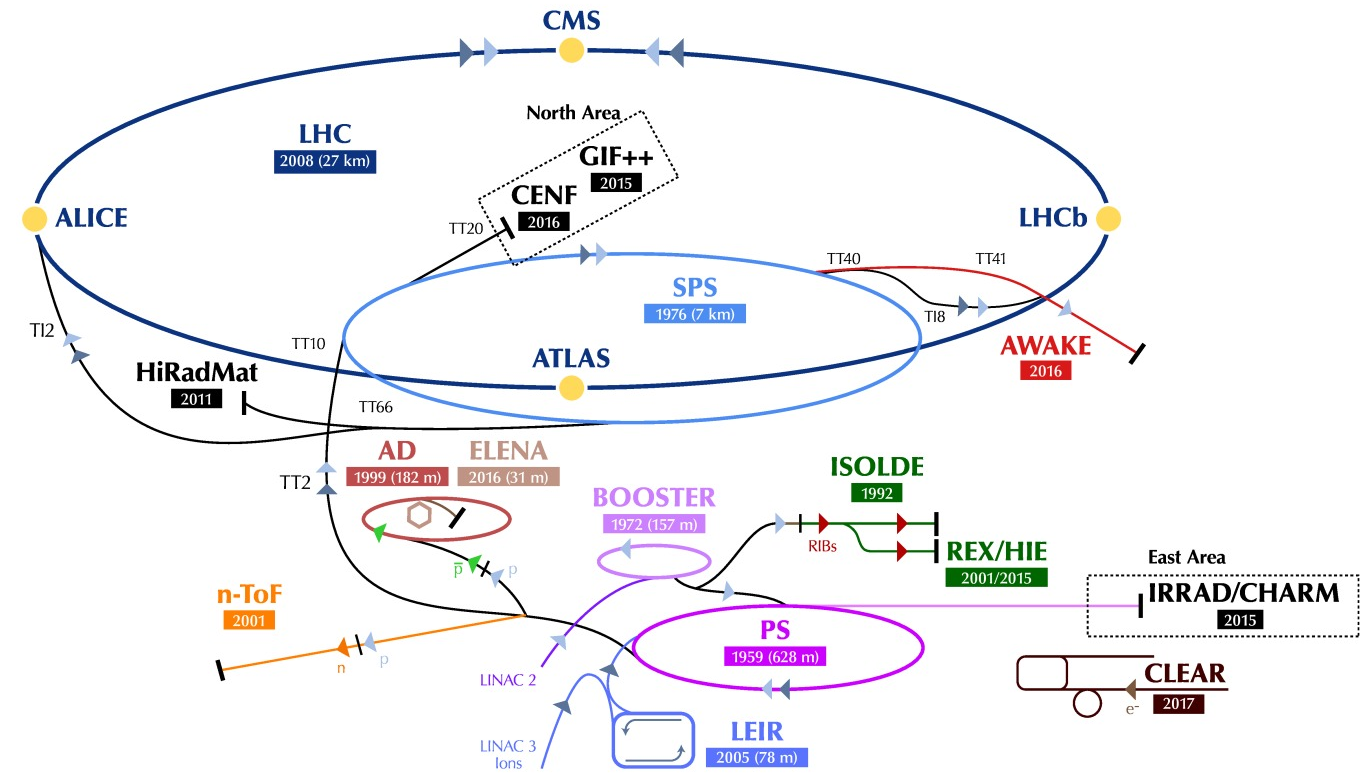
\includegraphics[width=0.8\linewidth]{ALICE/CernComplex_2018.png}   
        \caption{Complesso dell'intero acceleratore del CERN \\\small{Si vedono  \textcolor{blue}{LHC \textit{Large Hadron Collider}} \textcolor{cyan}{SPS \textit{Super Proton Synchrotron}} \textcolor{purple}{ PS \textit{Proton Synchrotron}} \textcolor{violet}{BOOSTER \textit{ Proton Synchrotron Booster}} LINAC \textit{Linear ACcelerator}} \\{\footnotesize  \textcolor{red}{AD \textit{Antiprotron Decelerator}} \textcolor{green}{ISOLDE \textit{Isotope Separator Online DEvice}}  \textcolor{lightgray}{LEIR \textit{Low Energy Ion Ring}} }}
        \label{fig:CERNcomplex}
    \end{figure}
    
Il fascio di particelle viaggia in un tubo in cui viene fatto l'ultra-vuoto ed è direzionato da dei magneti superconduttivi che devono essere tenuti alla temperatura di 1.85 $K$.

\section{ALICE}

L'acronimo ALICE sta per \textit{"A Large Ion Collider Experiment"} e lo  scopo primario dell'esperimento è quello di studiare la materia nucleare ad alte densità e alte temperature in uno stato chiamato \textit{quark-gluon plasma} (QGP). Il QGP è caratterizzato da quarks e gluoni liberi e non confinati negli adroni dalla forza nucleare forte. ALICE è ottimizzato per lo studio delle collisioni ad energie ultra-relativistiche di ioni pesanti (come il Piombo). L'obbiettivo dello studio del QGP è di comprendere le proprietà di questo stato della materia, la cui esistenza è prevista dalla cromodinamica quantistica, e di comprendere come si è formata la materia ordinaria, dato che si suppone che fino a $10^{-6}$ s dopo il Big-Bang esistesse solo questo stato della materia.  
    
    \begin{figure}[htbp]
        \centering
        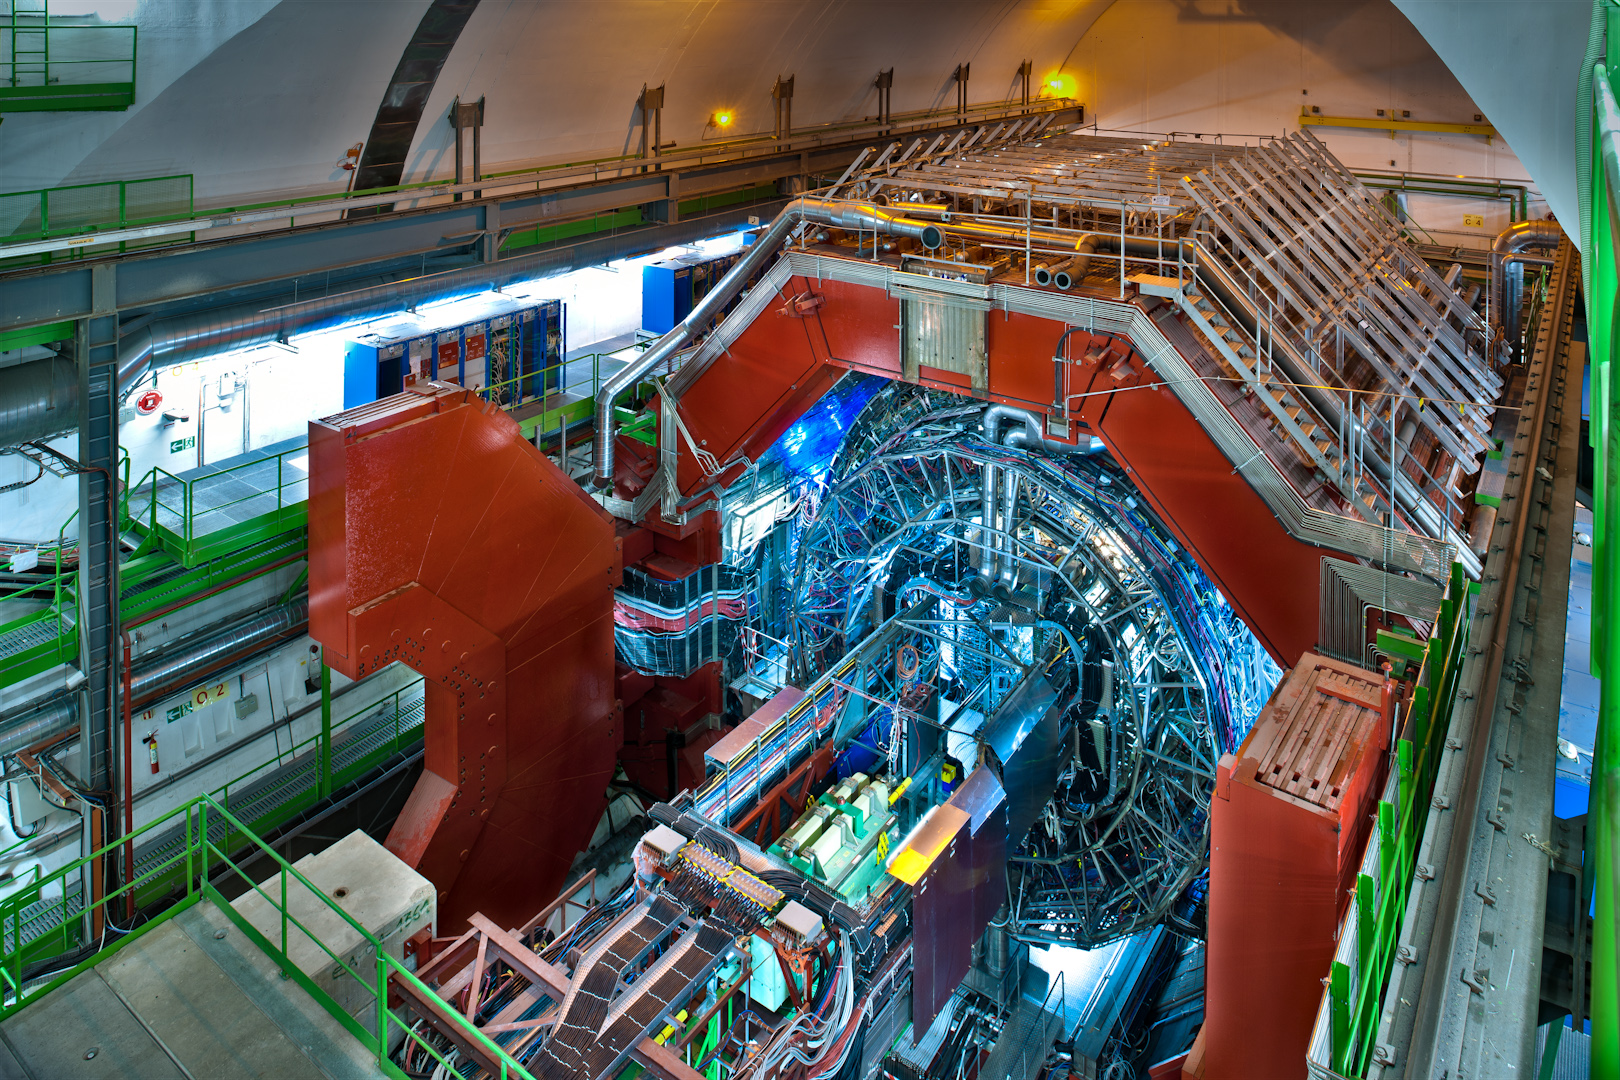
\includegraphics[width=0.6\linewidth]{ALICE/ALICE_LRsaba_CERN_0212_3219.jpg}
        \caption{Foto del rivelatore ALICE}
        \label{fig:ALICEcomplex}
    \end{figure}
    
ALICE \cite{Collaboration_2008_ALICE} è a sua volta composto da vari rivelatori di particelle che permettono di tracciare le traiettorie delle particelle prodotte nella collisione dei fasci, identificarle e misurarne velocità o momento. Si descrivono alcuni rivelatori di ALICE, i cui dati sono stati utilizzati ai fini di questa tesi.

    \subsection{Inner Tracking System (ITS)} \label{ITS}
    L'\textit{Inner Tracking System} è un rivelatore composto da sei cilindri concentrici di rivelatori in silicio di raggio minimo 3.9 $cm$ e massimo 43.0 $cm$, posizionati con l'asse parallelo alla direzione del fascio. Viene utilizzato per:
    \begin{itemize}
        \item la determinazione della posizione del vertice primario, cioè il punto in cui avviene la collisione; %Quest'ultimo è il punto in cui decade una particella generata nella collisione dei fasci, i cui prodotti possono poi decadere a loro volta (in questo caso il punto di decadimento è chiamato vertice secondario). %è una definizione esatta del vertice primario?
        \item la ricostruzione dei vertici secondari di decadimenti di particelle che decadono per interazione debole; 
        \item migliorare la precisione di tracciamento della Time Projection Chamber (TPC) (di cui si parla in seguito al \ref{TPC})
        \item permettere il tracciamento di particelle a basso momento che non vengono tracciate dalla TPC;
        \item identificazione di particelle (PID) con basso momento trasverso sfruttando la perdita specifica di energia $dE/dx$.
    \end{itemize}
    
    I rivelatori dell' ITS hanno una risoluzione spaziale di poche decine di micrometri. 
    
    \subsection{Time Projection Chamber  (TPC)} \label{TPC}
    La \textit{Time Projection Chamber}  è il miglior rivelatore di ALICE per la ricostruzione delle tracce delle particelle prodotte nella collisione. Si tratta di un rivelatore a gas di forma cilindrica, posizionato attorno all'ITS, con raggio interno di 85 $cm$ e esterno di 250 $cm$ e una lunghezza di 500 $cm$ nella direzione del fascio di particelle. Il raggio interno è determinato dalla massima densità di tracce accettabile dalla TPC, quello esterno dalla lunghezza minima necessaria per una precisione del 10$\%$ sulla perdita specifica di energia $dE/dx$. 
     
     \begin{figure}[htbp]
        \centering
        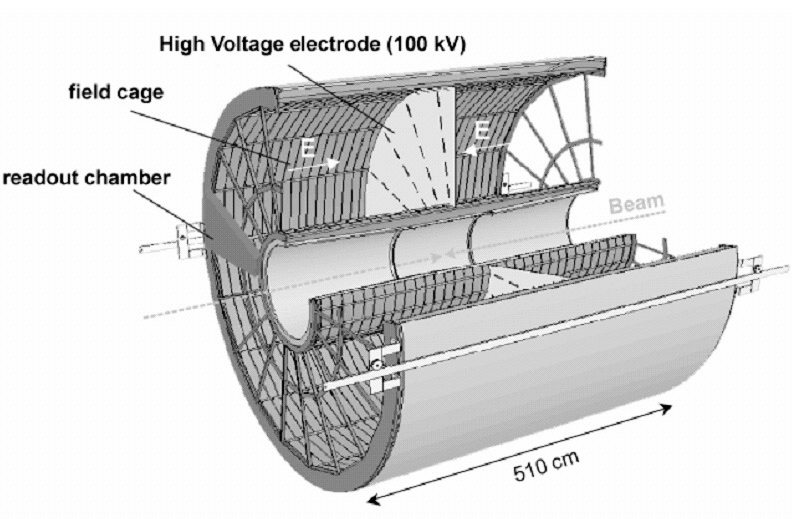
\includegraphics[width=0.7\linewidth]{ALICE/ALICE-TPC-detector.png}
        \caption{Schema della Time Projection Chamber di ALICE}
        \label{fig:TPCcomplex}
    \end{figure}
    
    La camera del TPC è riempita con una miscela di gas, che serve per trasportare gli elettroni di ionizzazione creati dal passaggio della particella da tracciare. Gli elettroni di ionizzazione vengono accelerati dal campo elettrico creato dagli elettrodi della TPC per arrivare alle placche esterne che permettono di registrare il segnale. \cite{Collaboration_2008_ALICE}
    \\La TPC è utilizzata per identificare le particelle tramite la misura della perdita specifica di energia per ionizzazione ($\frac{dE}{dx}$) e per la misura del momento. 
    
    %AGGIUNGERE TOF!
    
    \subsection{Time-Of-Flight (TOF)} \label{TOF}
    Il rivelatore Time-Of-Flight ha forma cilindrica, con raggio minimo di 370 cm e massimo di 399 cm. Questo rivelatore permette di misurare il tempo di volo delle particelle all'interno dei moduli di cui è composto e questa informazione viene utilizzata per l'identificazione della particella. Vale la relazione:
        \begin{equation}
            m = p\sqrt{\frac{t^2_{TOF}}{L^2}-1}
        \end{equation}
    dove $m$ è la massa della particella, $p$ il suo impulso, $t_{TOF}$ il tempo di volo e $L$ la lunghezza della traccia considerata. La risoluzione del rivelatore TOF è di 80 ps per pioni con momento di circa $1 GeV/c$ in collisioni Pb-Pb.
    Questo rivelatore viene utilizzato per l'identificazione di particelle (PID), in particolare di pioni e Kaoni con impulso fino a $2.5 \ GeV/c$ . La figura \ref{fig:TOF} mostra la distribuzione di $\beta = \frac{v}{c}$ misurata in funzione dell'impulso. 
    \begin{figure}[htbp]
        \centering
        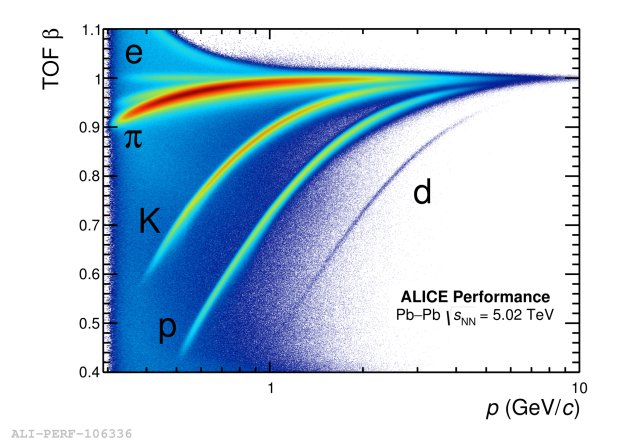
\includegraphics[width=0.8\linewidth]{ALICE/beta.png}
        \caption{Distribuzione della velocità $\beta = \frac{v}{c}$ misurata dal TOF in funzione dell'impulso, ottenuta dai dati di collisioni Pb-Pb con energia nel centro di massa $\sqrt{s} = 5.02 TeV$}
        \label{fig:TOF}
    \end{figure}
    
    